\documentclass[11pt]{article}
\input{commandPlotResults.tex}
\usepackage[frenchb,english]{babel}
\usepackage[margin=15mm]{geometry}
\usepackage{graphicx}
 \usepackage{color}
\usepackage{multirow}
\usepackage{multicol}
\usepackage{tikz}
\usepackage{adjustbox}
\usepackage{lscape}
\usepackage{float}
\usepackage{array}
\usepackage{calc}
\usepackage{amsmath}
\usepackage{dsfont}
\usepackage{hyperref}
\usepackage{tocloft}
\usepackage{titlesec}
\usepackage[scaled=.90]{helvet}
\usepackage{booktabs}
% Options pour les liens hypertexte
\hypersetup{
       backref=true,                           % Permet d'ajouter des liens dans
       pagebackref=true,                       % les bibliographies
       hyperindex=true,                        % Ajoute des liens dans les index.
       colorlinks=true,                        % Colorise les liens.
       breaklinks=true,                        % Permet le retour à la ligne dans les liens trop longs.
       urlcolor= black,                         % Couleur des hyperliens.
       linkcolor= black,                        % Couleur des liens internes.
       citecolor=black,			% Couleur pour les liens de biblio
       bookmarks=true,                         % Créé des signets pour Acrobat.
       bookmarksopen=true,                     % Si les signets Acrobat sont créés,
                                               % les afficher complètement.
       pdftitle={},  % Titre du document.
                                               % Informations apparaissant dans
       pdfauthor={Sebastien Benzekry},                      % dans les informations du document
       pdfsubject={Mathematics}           % sous Acrobat.
    }

\titleformat{\section}
  {\normalfont\sffamily\Large\bfseries}
  {\thesection}{0em}{}

\newcounter{fignb}  % to number supplementary figures 
\newcounter{tabnb} % to number supplementary tables
%-----------------------------------------------------------
%-----------------------------------------------------------
%-----------------------------------------------------------
\begin{document}
\renewcommand\thesection{}
\renewcommand\thesubsection{}
\renewcommand\thesubsubsection{}
\fontfamily{phv}\selectfont
\pagenumbering{gobble}
%-----------------------------------------------------------%%%
\graphicspath{
{/Users/benzekry/work/marseille/neuroblastome_andre/code/}
{figures_files/}
}
%-----------------------------------------------------------%%%
\setlength{\parindent}{0mm}
%-----------------------------------------------------------%%%
\textbf{\Huge{Supplementary figures and tables}}

\renewcommand{\cfttoctitlefont}{\normalfont\MakeUppercase}
\renewcommand{\contentsname}{}
\tableofcontents

\vskip2cm
%-----------------------------------------------------------%%%
\newpage
\vskip2cm
\renewcommand\thesection{}
%-----------------------------------------------------------
\def\spaceV{\vskip0.5cm}
\pagenumbering{gobble}
%-----------------------------------------------------------
%-----------------------------------------------------------
\newpage
\stepcounter{tabnb}
\section{Table S\arabic{tabnb}: Neuroblastoma classification according to the International Neuroblastoma Risk Group staging system}
\spaceV
\begin{center}
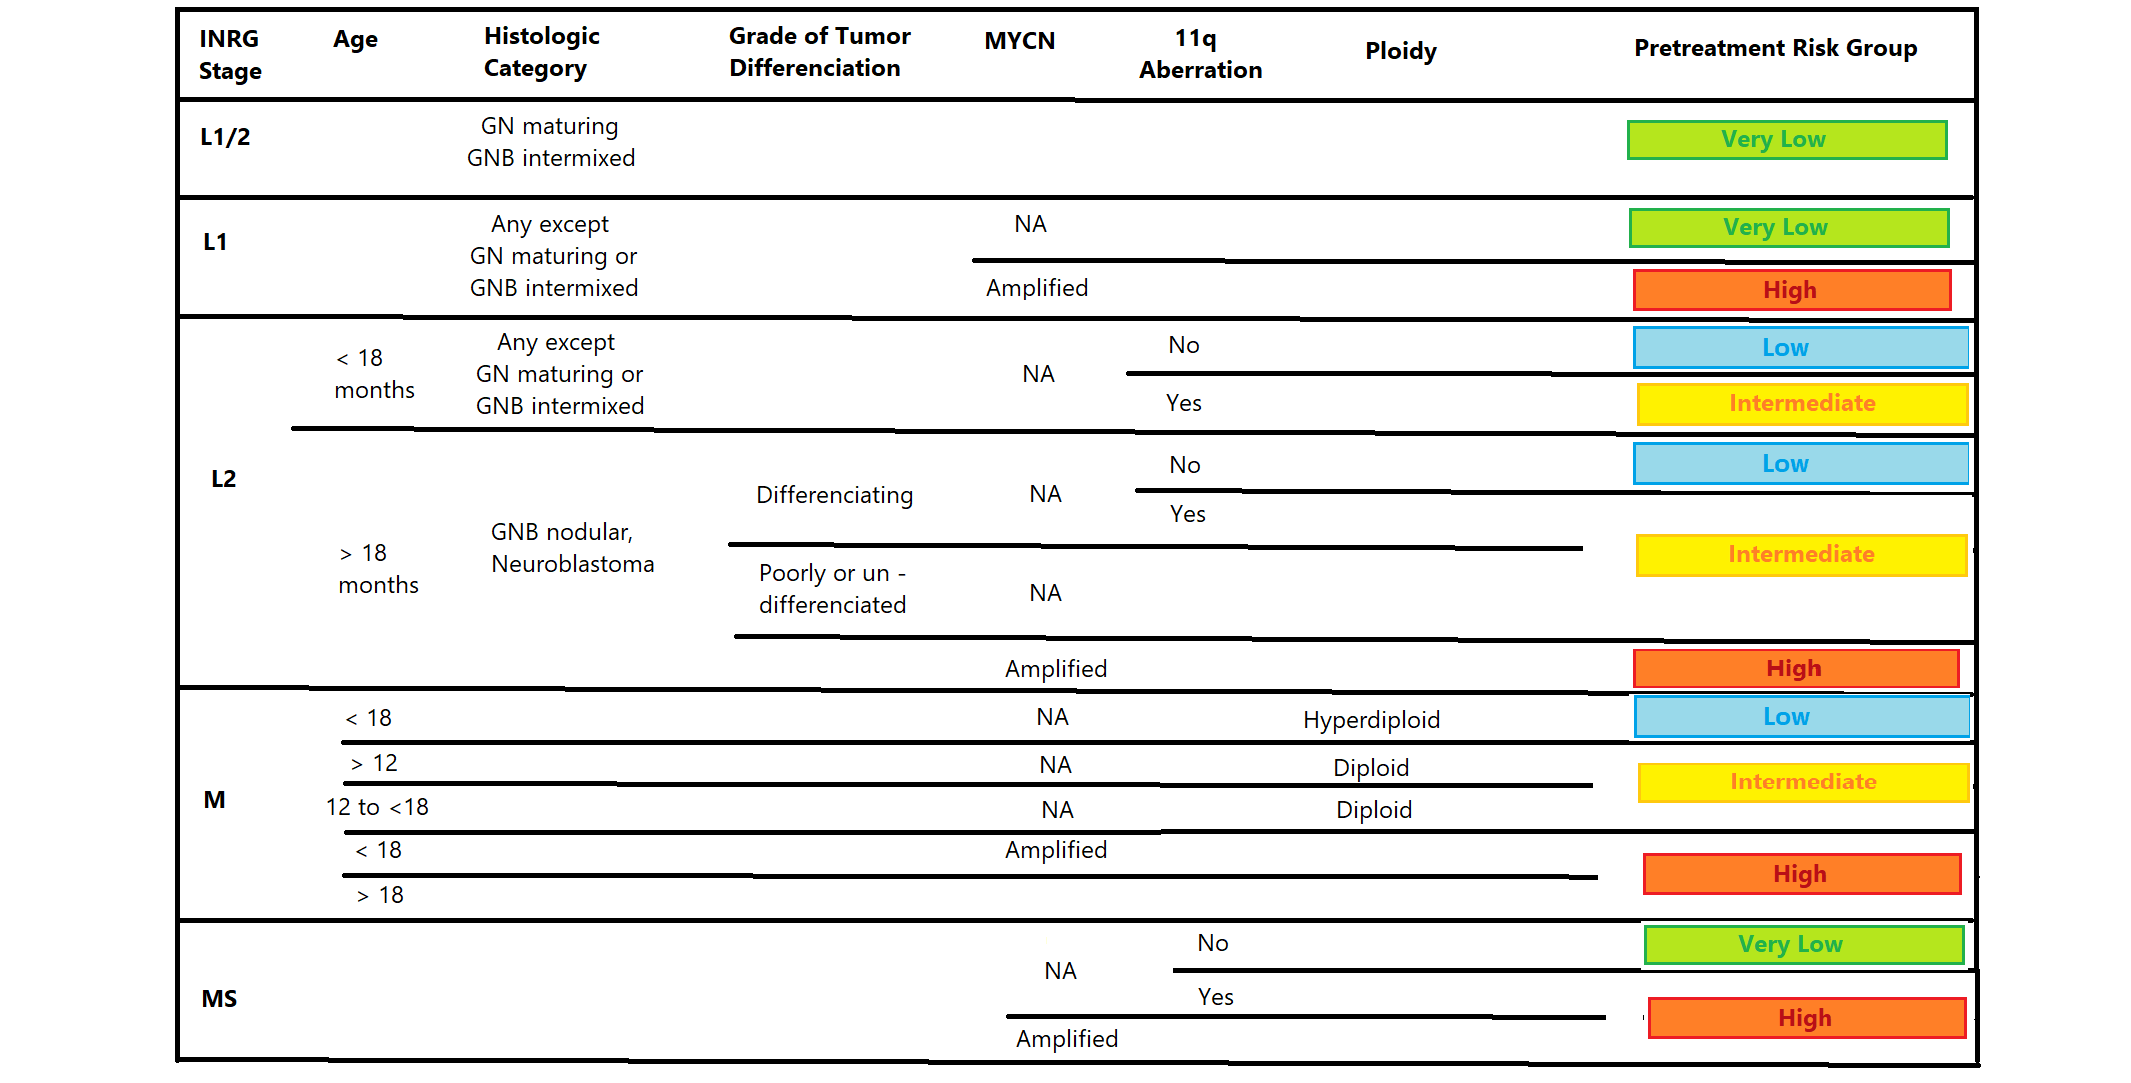
\includegraphics[width=1\textwidth]{table_S1}
\end{center}
Adapted from ref [6]. GN: Ganglioneuroma. GNB: Ganglioneuroblastoma. NA: Non Amplified.
%-----------------------------------------------------------
\newpage
\stepcounter{tabnb}
\section{Table S\arabic{tabnb}: Cox analysis of progression-free survival}
\spaceV
\begin{center}
\begin{tabular}{lrrrr}
\toprule
{} &  Hazard ratio &      p &  coef lower 95\% &  coef upper 95\% \\
covariate  &               &        &                  &                  \\
\midrule
age        &             1 &  0.758 &            0.983 &             1.02 \\
sex        &           1.6 &   0.33 &            0.621 &             4.13 \\
log(LDH)   &          2.21 & 0.0617 &            0.962 &             5.07 \\
SIOPEN     &             1 &  0.847 &            0.973 &             1.03 \\
MYCN       &         0.604 &  0.498 &            0.141 &             2.59 \\
tumor size &             1 &  0.114 &                1 &                1 \\
\bottomrule
\end{tabular}

\end{center}
%-----------------------------------------------------------
\newpage
\stepcounter{fignb}
\section{Figure S\arabic{fignb}: HRNBL1 protocol}
\spaceV
\begin{center}
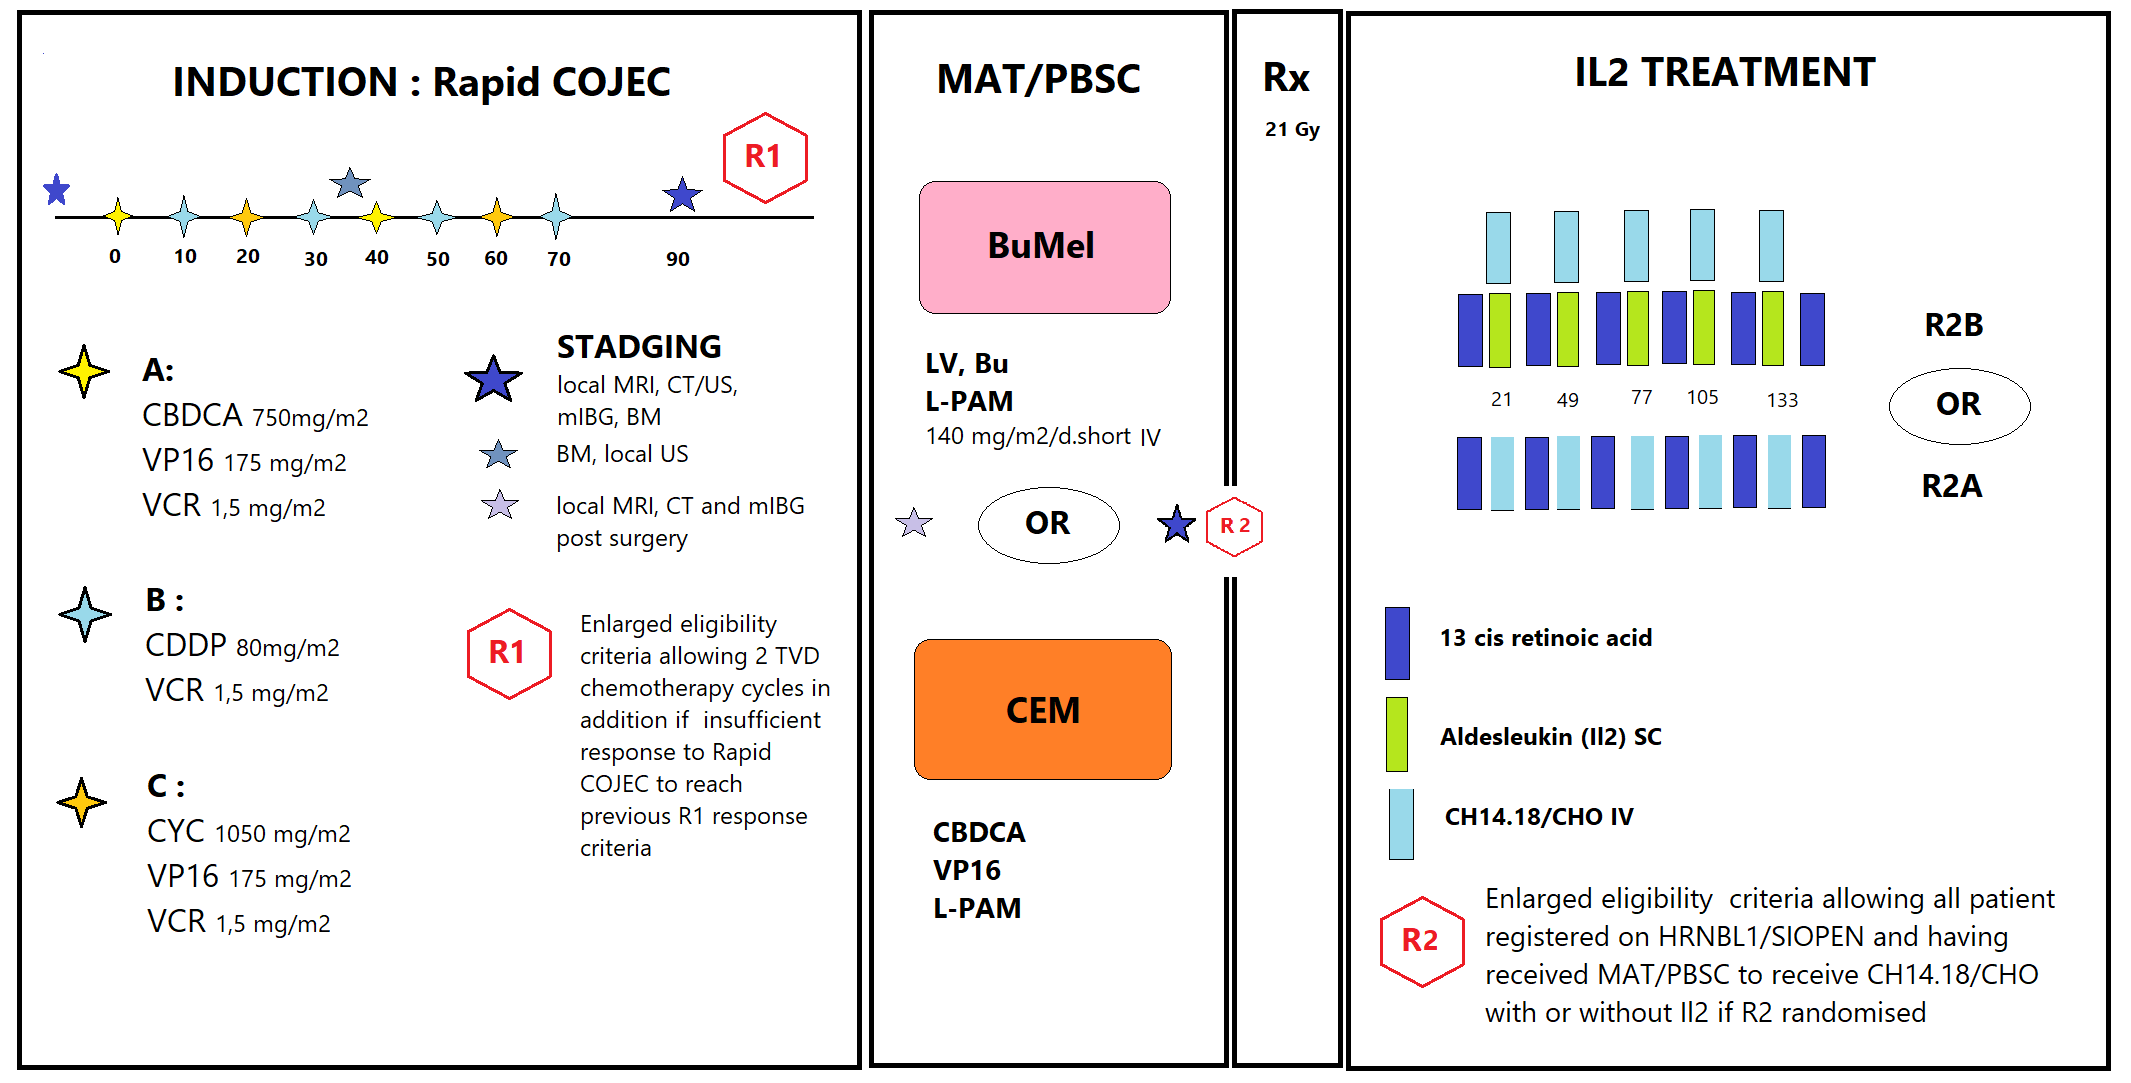
\includegraphics[width=1\textwidth]{figure_S1}
\end{center}

Time is in days.\\
Staging: MRI: Magnetic Resonance Imaging. CT: Computerized tomography. US: Ultrasound. mIBG: meta-iodo-benzyl-guanidine scintigraphy. BM: Medullar Bone exploration.\\
Treatments: COJEC: Chemotherapy protocol including C Cisplatin, O Vincristine, J Carboplatin, E Etoposide and C Cyclophosphamide given in rapid delivery schedule. CBDCA: Carboplatine, VP16: Etoposide, VCR: Vincristine, CDDP: Cisplatin, CYC Cyclophosphamide. MAT: Myeloablative therapy. PBSC: Peripherical Blood Stem Cell. Bu Mel: Busulphan Mephalan. L-PAM : Melphalan. CEM : Carboplatine Etoposide Melphalan MAT Regimen. Rx: Radiotherapy. SC : subcutaneous / IV : intravenous

CH14.18/CHO: anti-GD2 chimeric monoclonal antibody.
%-----------------------------------------------------------
\newpage
\stepcounter{fignb}
\section{Figure S\arabic{fignb}: SIOPEN scoring}
\spaceV
\begin{center}
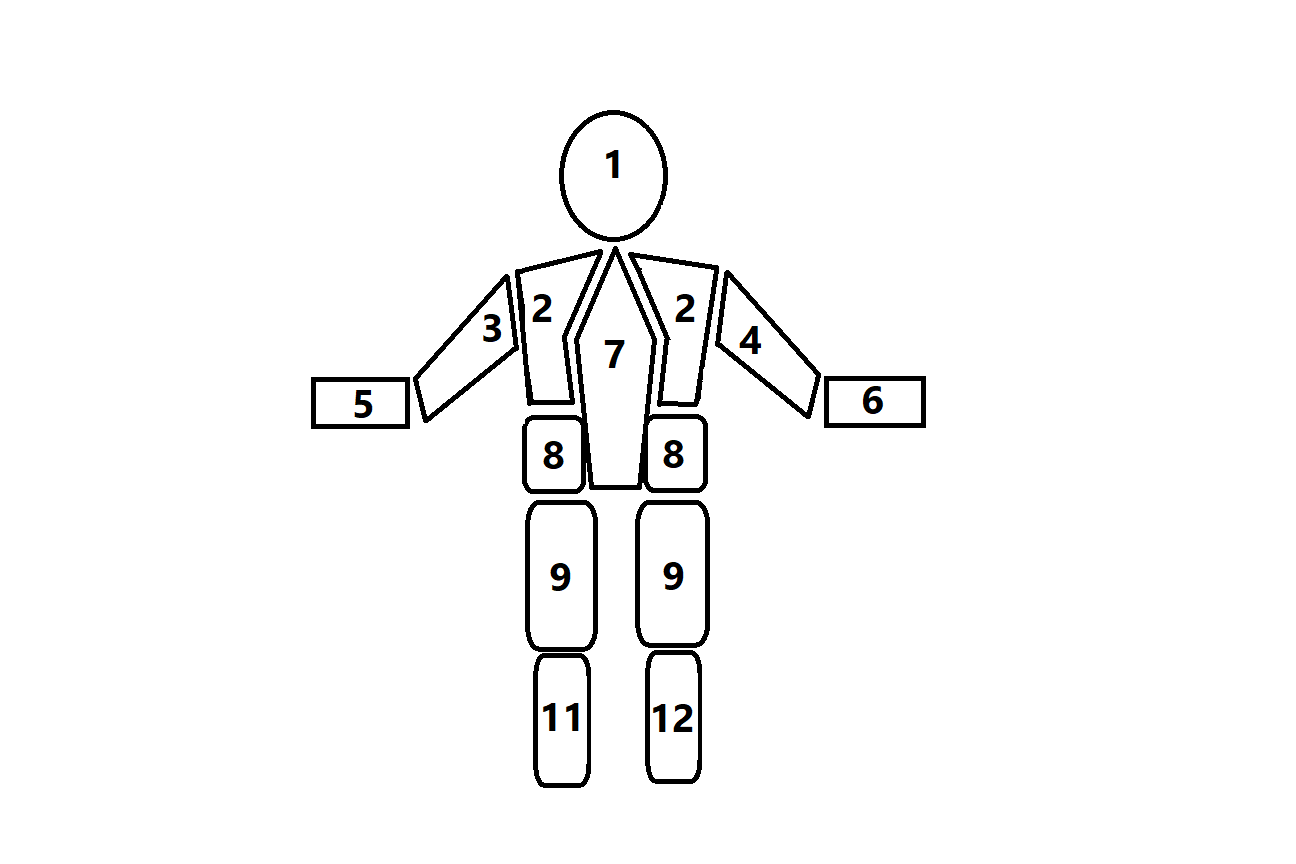
\includegraphics[width=1\textwidth]{figure_S2}
\end{center}
To score patients, the skeleton is divided into 12 segments, and for each of them extension of the lesions is scored as:
\begin{itemize}
\item 0: no lesion
\item 1 for 1 lesion
\item 2 for 2 lesions
\item 3 for 3 lesions
\item 4 for $>$ 3 lesions but $< 50\%$ of the concerned segment
\item 5 for diffuse disease but $<95\%$ of the whole segment
\item 6 for difsuse disease $>95\%$ of  whole segment
\end{itemize}
The SIOPEN score is then defined as the sum of each segment's score.
%-----------------------------------------------------------
\newpage
\stepcounter{fignb}
\section{Figure S\arabic{fignb}: Primary tumor and metastases location}
\spaceV
\begin{center}
\textbf{A}
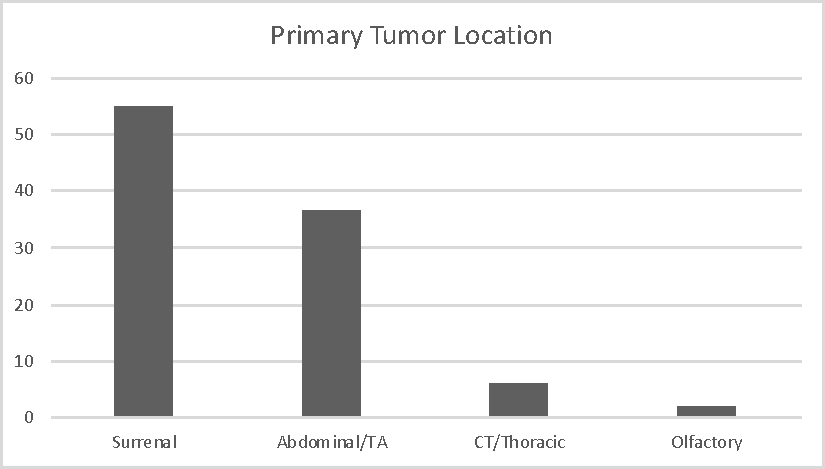
\includegraphics[width=0.45\textwidth]{primary_location}
\textbf{B}
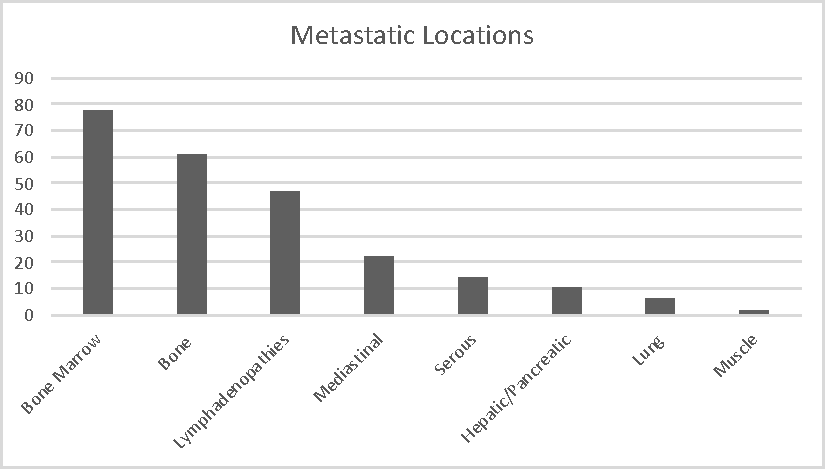
\includegraphics[width=0.45\textwidth]{metastatic_locations}
\end{center}
%-----------------------------------------------------------
\newpage
\stepcounter{fignb}
\section{Figure S\arabic{fignb}: Simulations of all patients}
\spaceV
\begin{center}
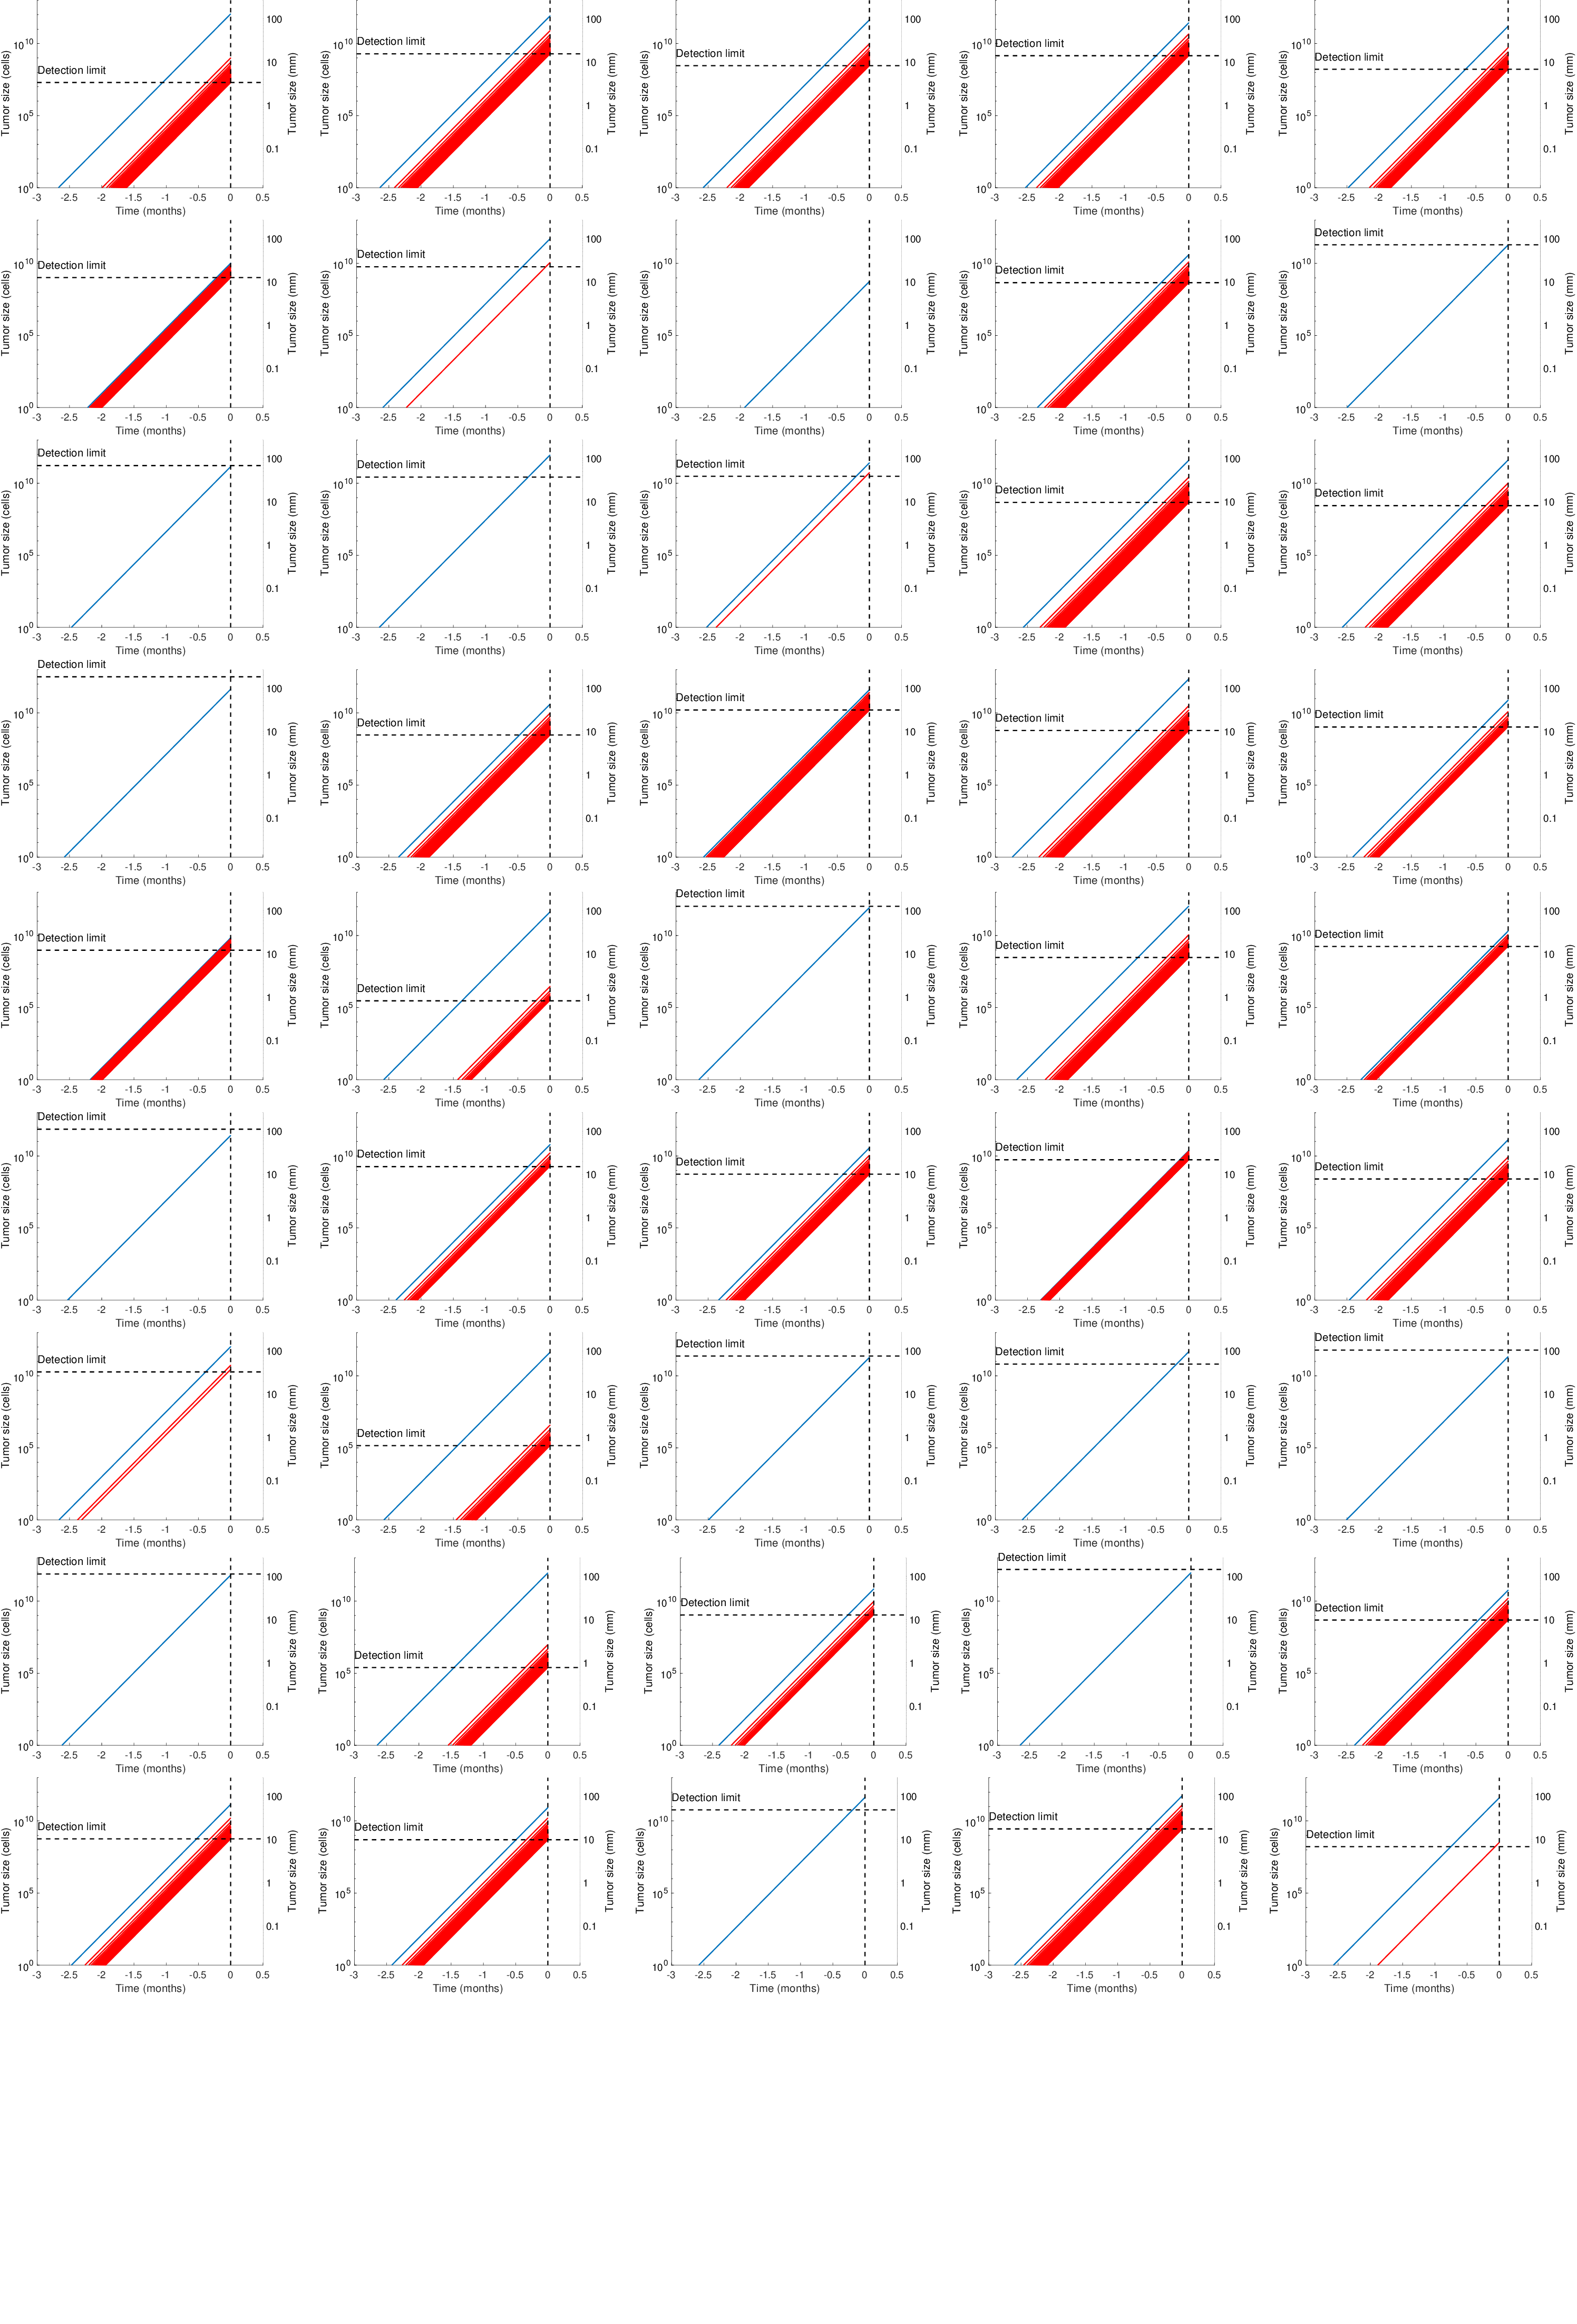
\includegraphics[width=0.8\textwidth]{all_plots.png}
\end{center}

Simulations of the mechanistic model for all patients in the cohort. Blue line is the size of the primary tumor. Red lines are the predicted sizes of the metastases.
%-----------------------------------------------------------
\newpage
\stepcounter{fignb}
\section{Figure S\arabic{fignb}: Overall survival analysis in dichotomized groups}
\spaceV
\begin{center}
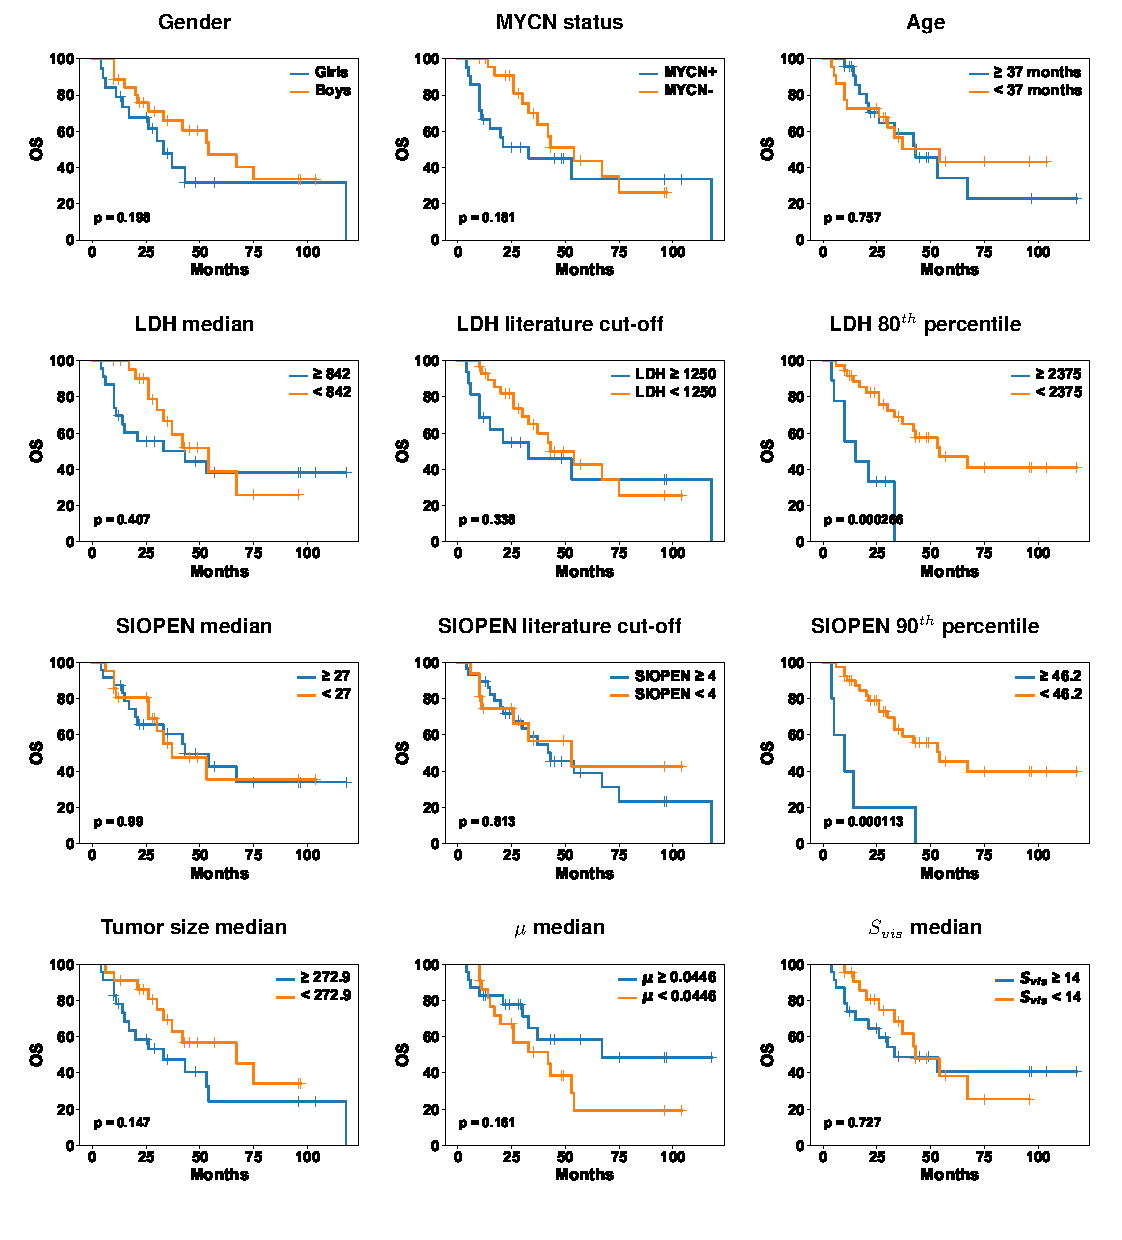
\includegraphics[width=1\textwidth]{figure_S5}
\end{center}
Dichotomized analysis of overall survival (OS) according to the different variables, at median or literature cut-offs.
%-----------------------------------------------------------
\newpage
\stepcounter{fignb}
\section{Figure S\arabic{fignb}: Progression-free survival analysis in dichotomized groups}
\spaceV
\begin{center}
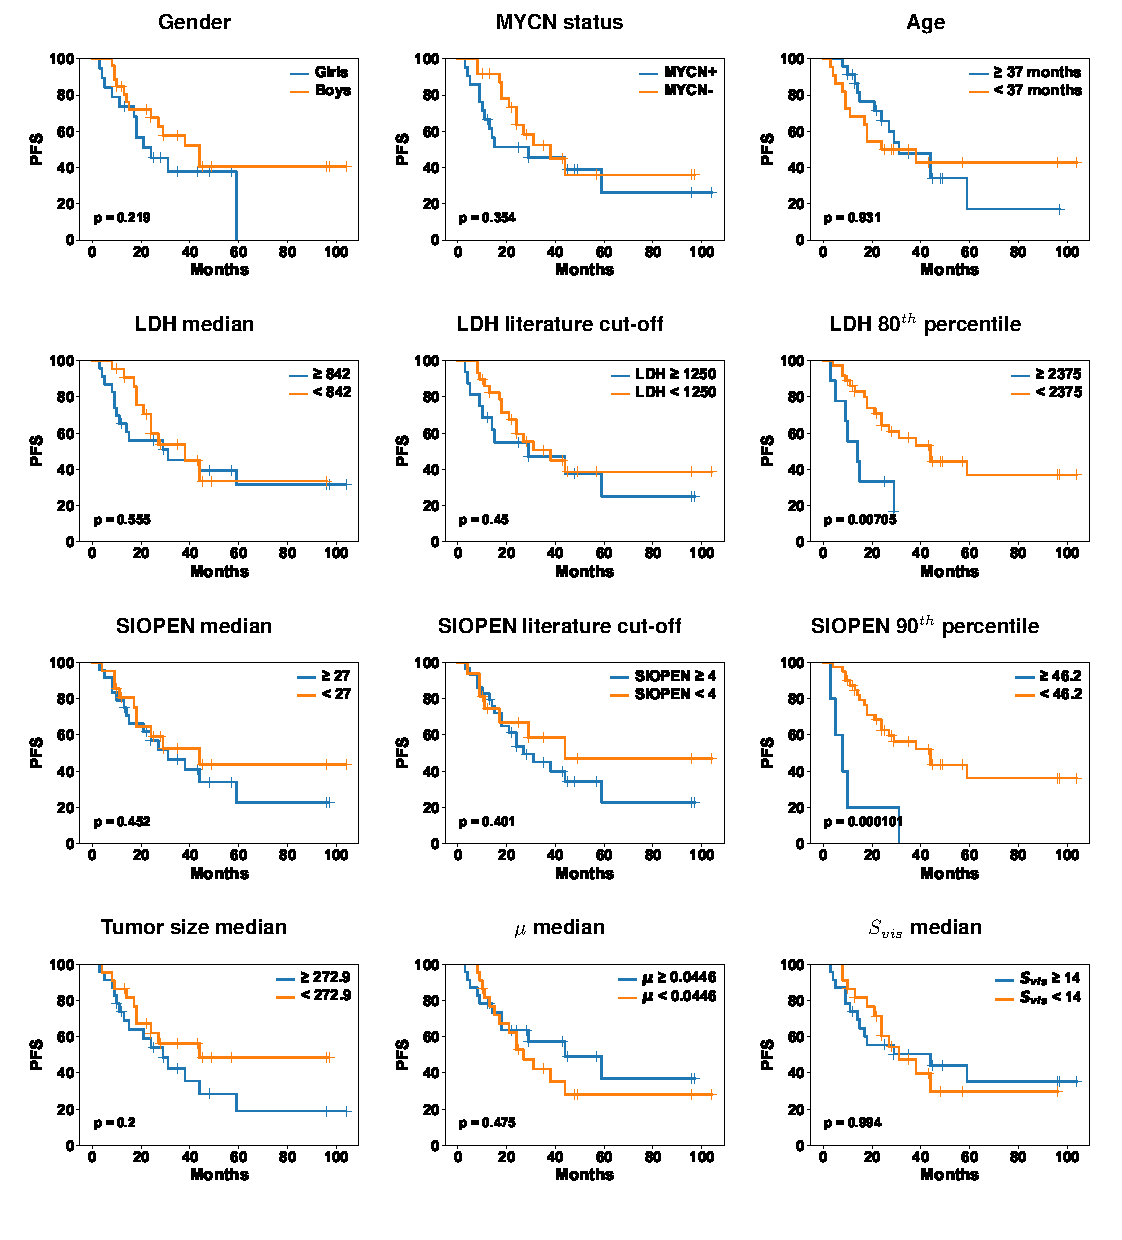
\includegraphics[width=1\textwidth]{figure_S6}
\end{center}
Dichotomized analysis of progression-free survival (PFS) according to the different variables, at median or literature cut-offs.
%-----------------------------------------------------------
\newpage
\stepcounter{fignb}
\section{Figure S\arabic{fignb}: Calibration plots}
\spaceV
\begin{center}
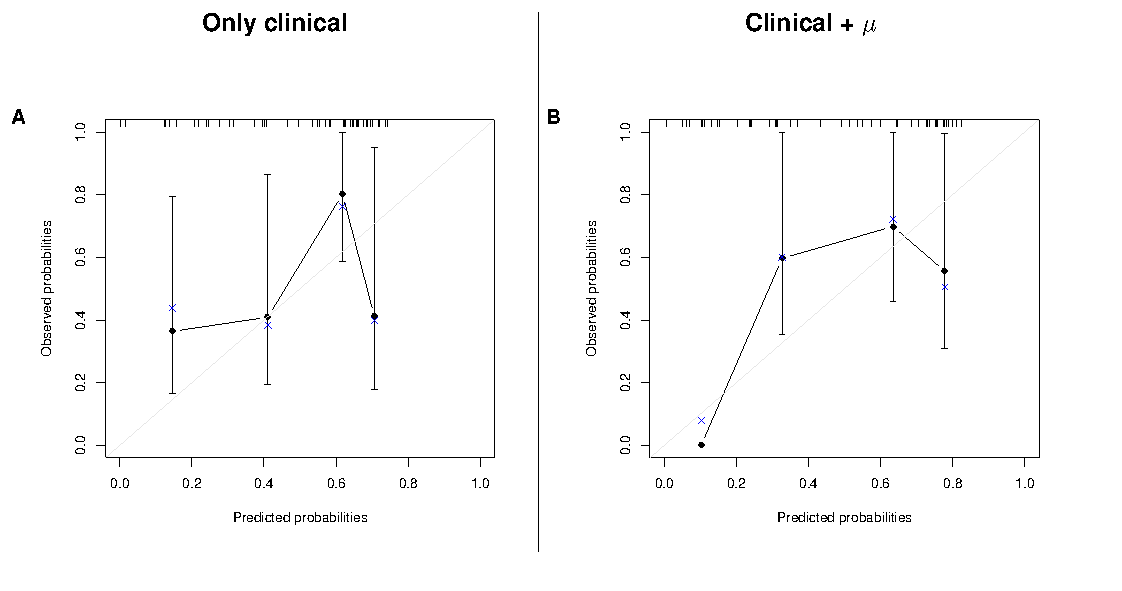
\includegraphics[width=1\textwidth]{figure_S7}
\end{center}
A. Calibration plots of the prediction model with only clinical variables (i.e. tumor size and log(LDH) after variable selection). Crosses mark the bootstrap corrected estimates.
B. Same as A. for the prediction model using the mathematical biomarkers as additional variables in the model (i.e. $\log(\mu)$ and log(LDH)) after variable selection).
\end{document}